\section{System}
\label{sec:system}

\begin{figure}[t]
  \centering
  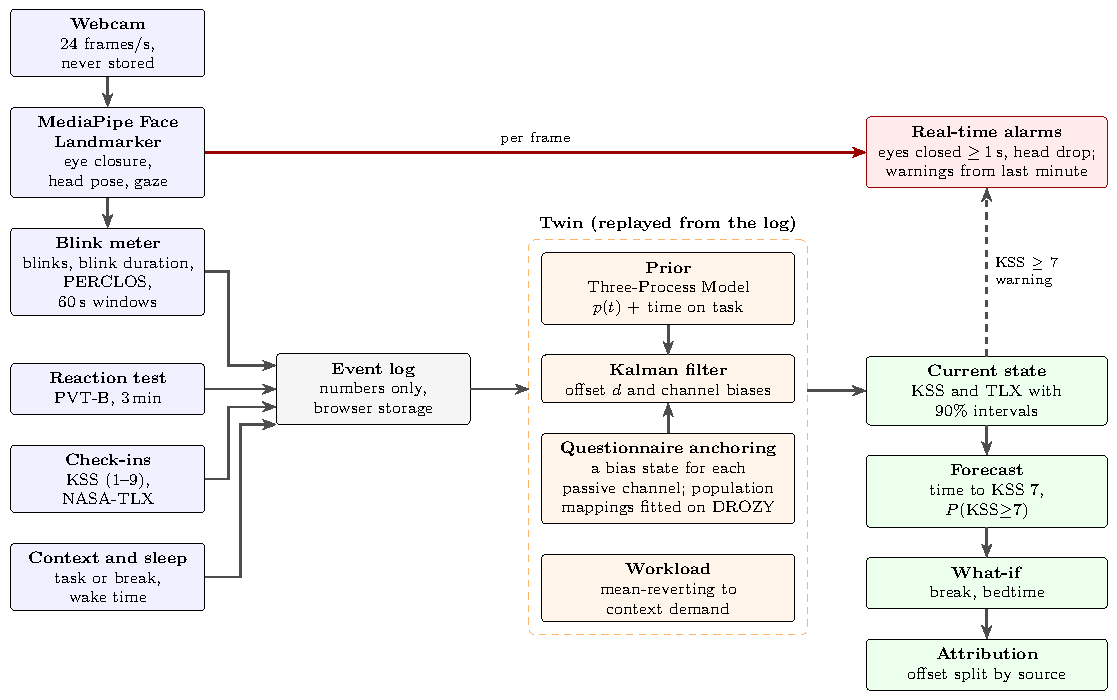
\includegraphics[width=\linewidth]{figures/architecture.pdf}
  \caption{BlinkTwin architecture. Webcam frames are processed in the page and discarded. Per frame, eye closure and head pose drive real-time alarms. Per minute, a summary of the eyes is stored as an event, together with reaction-test results, check-ins and context entries. The twin's state at any time is rebuilt by replaying these events through one Kalman filter.}
  \label{fig:architecture}
\end{figure}

BlinkTwin is a single-page web application written in TypeScript (Figure~\ref{fig:architecture}). It needs a laptop with a webcam and a current browser, and nothing is installed. All computation runs in the page.

\subsection{Webcam sensing}
Frames from the webcam are passed, at up to 24 per second, to the MediaPipe Face Landmarker \citep{kartynnik2019real,lugaresi2019mediapipe} in video mode, with one face, blendshapes and the facial transformation matrix enabled. For each frame the eye-closure score $c_t$ is the mean of the \texttt{eyeBlinkLeft} and \texttt{eyeBlinkRight} blendshapes (0 = open, 1 = closed), or missing when no face is found.

The open-eye level of this score differs between people, cameras and lighting, so the \emph{blink meter} normalises it against the person's own recent baseline. With $b_t$ the 20th percentile of $c$ over the previous 30~s,
\begin{equation}
  \hat c_t = \min\!\left(1, \max\!\left(0, \frac{c_t - b_t}{1 - b_t}\right)\right).
\end{equation}
A closure starts when $\hat c_t \geq 0.5$ and ends when $\hat c_t \leq 0.3$ (hysteresis). Closures lasting 50--1000~ms are counted as blinks; longer ones are counted separately as long closures. Every 60~s the meter reports the blink rate, the mean blink duration, the number of long closures, PERCLOS (the fraction of frames with a face in which $\hat c_t \geq 0.8$) and coverage (the fraction of frames with a face). These per-minute windows are the only camera data that are stored. The same blink meter, unchanged, was run on landmark data from DROZY and validated against the electro-oculogram (Section~\ref{sec:grounding}).

\paragraph{Head pose and gaze.} Pitch, yaw and roll are computed from MediaPipe's facial transformation matrix and expressed relative to the person's resting pose, the median of the last 20~s. A head nod is a pitch deviation of at least 12$^\circ$ that returns within 2.5~s. Gaze direction is estimated from the \texttt{eyeLook} blendshapes. The interface draws the eye landmarks over the live video and plots eye closure and head pitch for the last 30~s, so the person can see what the camera measures. Nods and head movement are stored with each window; they are not yet used by the twin.

\subsection{Real-time alarms}
A rule-based monitor runs on every frame, independently of the twin's minute-level state. It raises an \emph{alarm} (red, with a sound) when the eyes stay closed continuously for at least 1.0~s, or when the head has dropped from its resting pitch for at least 1.0~s while the eyes are at least half closed; these are signs of a microsleep. The alarm clears after the eyes have been open for 1.5~s. It raises a \emph{warning} (amber) when, over the last minute, PERCLOS is at least 15\%, there are at least two closures longer than 1~s, the mean blink duration is at least 300~ms with at least five blinks, or the twin's KSS estimate reaches 7; warnings repeat at most every 5~minutes. These thresholds are defaults chosen from the literature cited in Section~\ref{sec:related}. They have not been validated, and their sensitivity to microsleeps against EOG or video ground truth is an outcome of the validation study (Section~\ref{sec:protocol}).

\subsection{Reaction-time test}
The reaction test follows the PVT-B \citep{basner2011validity}: 3~minutes, inter-stimulus intervals drawn uniformly from 1--4~s, a millisecond counter as the stimulus, and a response with the space bar, a click or a tap. The reaction time is shown for 600~ms as feedback. Responses with no stimulus on screen, or faster than 100~ms, are false starts; reaction times above 355~ms are lapses. The test reports the number of valid responses, the median reaction time, the mean response speed ($1000/\RT$), lapses and false starts. A 1-minute version is offered for convenience and is marked as less reliable. Browser and keyboard timing add a delay of a few milliseconds that is roughly constant within a device; the per-channel bias state of the twin absorbs such constant offsets.

\subsection{Check-ins}
A check-in asks for the KSS rating of the last 5~minutes, using the original verbal anchors \citep{akerstedt1990subjective}, and optionally the six NASA-TLX subscales for the task just done \citep{hart1988development}, each on a 0--100 slider in steps of 5. The raw TLX (the unweighted mean) is stored. After every reaction test the app asks for a check-in.

\subsection{Context and sleep}
The person can mark what they are doing (focused work, reading, a meeting, another task, or a break) and can enter the time they woke and how long they slept. Without these entries the twin assumes waking at 07:00 after 7.5~h of sleep.

\subsection{Event log and replay}
Every input is stored as a timestamped event: \texttt{sleep}, \texttt{context}, \texttt{kss}, \texttt{tlx}, \texttt{pvt}, \texttt{cam} and \texttt{alert}. The twin has no hidden state. Its estimate at any time is obtained by replaying the events up to that time through the model in Section~\ref{sec:model}. Every displayed number is therefore reproducible from the log, and the website, the 24 unit tests and the simulation study run exactly the same code.

\subsection{Privacy}
Video frames exist only in memory for the duration of one model call. No image, landmark or blendshape trace is stored. Events are kept in the browser's local storage and can be exported (CSV or JSON) or deleted by the person. The application sends no personal data over the network; the only network traffic is loading the application and, on first use, the MediaPipe model file.
